次に,Ahmed Bluff Bodyと呼ばれる次の図\ref{fig:ahmed-body}のようなモデルを用いて,シミュレーションをした.
このモデルは,CFDのベンチマークとして用いられるモデルであり,
抵抗係数$Cd$,浮力係数$Cl$が次の表\ref{tab:ahmed-cd-cl}のように知られている\cite{ref:ahmed-bluff-body}.
今回は,動せん断粘度$\nu=\SI{2.5E-6}{\square\meter\per\second}$,最大レイノルズ数$Re=5.89E7$,
シミュレーション時間は$\SI{0.25}{\second}$としてシミュレーションをした.

得られた$Cd$の時間変化を図\ref{fig:ahmed-cd-t}に示す.
このうち,$Cd$の値を$0$から$1$までの範囲に限定したものを図\ref{fig:ahmed-cd-t-lim}に示す.

\begin{figure}[ht]
    \begin{minipage}{0.48\linewidth}
        \centering
        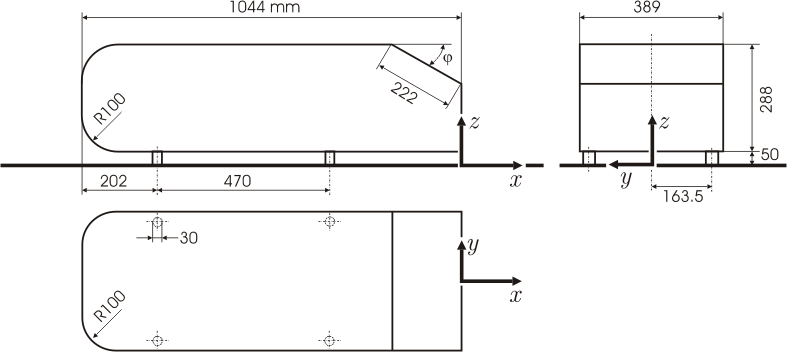
\includegraphics[width=\linewidth]{figures/ahmed/ahmed.png}
        \subcaption{設計図}
    \end{minipage}
    \begin{minipage}{0.48\linewidth}
        \centering
        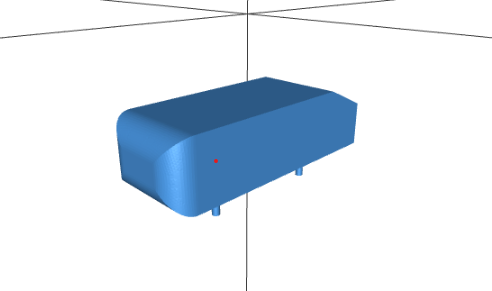
\includegraphics[width=\linewidth]{figures/ahmed/img.png}
        \subcaption{外観}
    \end{minipage}
    \caption{Ahmed Bluff Body}
    \label{fig:ahmed-body}
\end{figure}

\begin{table}[htbp]
    \centering
    \caption{Ahmed Bluff Bodyの抵抗係数$Cd$,浮力係数$Cl$}
    \begin{tabular}{ccc}
        \toprule
           & Cd    & Cl    \\
        \midrule
           & 0.300 & 0.316 \\
           & 0.266 & 0.325 \\
           & 0.274 & 0.33  \\
           & 0.250 & 0.306 \\
           & 0.260 & 0.305 \\
           & 0.301 & 0.307 \\
        \midrule
        平均 & 0.275 & 0.315 \\
        \bottomrule
    \end{tabular}%
    \label{tab:ahmed-cd-cl}%
\end{table}%

\begin{figure}[ht]
    \centering
    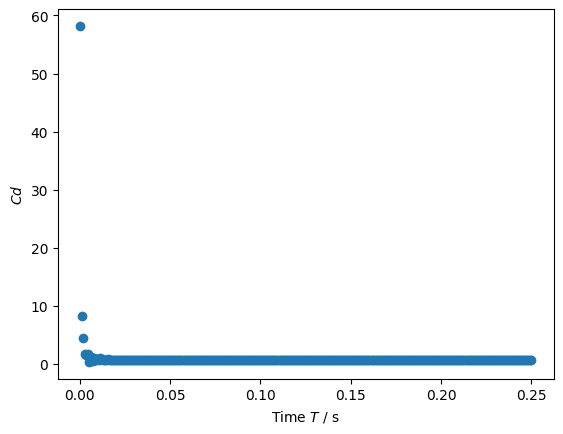
\includegraphics[width=0.8\linewidth]{figures/ahmed/ahmed-cd.png}
    \caption{AhmedBluffBodyの$Cd$の時間変化}\label{fig:ahmed-cd-t}
\end{figure}

\begin{figure}[ht]
    \centering
    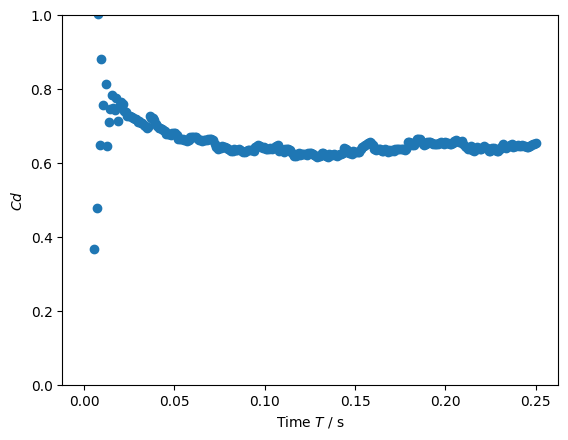
\includegraphics[width=0.8\linewidth]{figures/ahmed/ahmed-cd-0-1.png}
    \caption{AhmedBluffBodyの$Cd$の時間変化 拡大図}\label{fig:ahmed-cd-t-lim}
\end{figure}